\chapter{KẾT QUẢ THỰC NGHIỆM}
\label{chap:ketqua}

Chương này trình bày kết quả của bốn thí nghiệm: E1 đo độ chính xác phát hiện (gồm cả so sánh kiến trúc), E2 đo tốc độ,
E3 đo chất lượng theo dõi và sai số đếm xe, E4 phân tích các loại lỗi. Cuối chương là ứng dụng web, phần thảo luận và
kết luận. Mọi con số được lấy từ file kết quả của từng lần chạy.

\section{Tiêu chí và cách đánh giá}

\textbf{Phát hiện.} Chỉ số chính là mAP50 trung bình của xe máy và ô tô (mục~\ref{sec:chi-so}), kèm khoảng tin cậy
bootstrap 95\%. Mọi mô hình được chấm bằng cùng một đường chấm (pycocotools, ngưỡng tin cậy 0.001, tối đa 500 phát hiện
mỗi ảnh, có vùng bỏ qua), mỗi mô hình chạy ở đúng kích thước ảnh lúc huấn luyện. mAP50-95 chỉ được dùng trên các tập
mà nhãn sơ bộ không đến từ mô hình đang so sánh (\texttt{vn\_extra}, val UVH-26, UA-DETRAC); lý do ở
mục~\ref{sec:thao-luan}. Tập test Roboflow, val UVH-26 dùng cả bốn lớp; UA-DETRAC dùng xe máy, ô tô và xe buýt.

\textbf{Theo dõi.} Trên tập test (clip Phạm Văn Đồng) báo đủ HOTA, DetA, AssA, MOTA, IDF1, IDR, IDP và số lần đổi ID.
Trên tập dev VnTraffic chỉ dùng AssA, IDR và số lần đổi ID vì nhãn thiếu xe.

\textbf{Đếm xe.} So số lượt qua vạch theo lớp và hướng giữa hệ thống và nhãn tay.

\textbf{Tốc độ.} Thời gian xử lý mỗi frame (trung vị và khoảng tứ phân vị) trên CPU Intel Core i5-8250U và GPU Tesla T4.

\section{Kết quả phát hiện}
\label{sec:ket-qua-phat-hien}

\subsection{Tập test Hà Nội}

\begin{table}[H]
  \centering
  \caption{Kết quả phát hiện trên tập test Hà Nội (30 frame; 2.982 xe máy, 539 ô tô)}
  \label{tab:e1-hanoi}
  \small
  \begin{tabularx}{\linewidth}{|L|c|c|c|c|}
    \hline
    \thead{Mô hình} & \thead{Ảnh} & \thead{mAP50 chính [CI 95\%]} & \thead{AP50 xe máy} & \thead{AP50 ô tô} \\ \hline
    YOLO26n gốc COCO & 1280 & 0.686 [0.674--0.701] & 0.530 & 0.842 \\ \hline
    v1 & 640 & 0.395 [0.368--0.414] & 0.045 & 0.744 \\ \hline
    v2 & 960 & 0.890 [0.882--0.901] & 0.819 & 0.961 \\ \hline
    v3 & 960 & 0.921 [0.915--0.934] & 0.865 & 0.978 \\ \hline
    v4 & 1280 & 0.919 [0.910--0.927] & 0.862 & 0.975 \\ \hline
    \textbf{v5} & 960 & \textbf{0.923} [0.915--0.932] & 0.864 & 0.982 \\ \hline
  \end{tabularx}
\end{table}

Bảng~\ref{tab:e1-hanoi} cho thấy tinh chỉnh trên dữ liệu phù hợp nâng mAP50 chính từ 0.686 (mô hình gốc COCO, chạy ở
ảnh 1280) lên 0.923. Bước nhảy lớn nhất ở xe máy: AP50 từ 0.530 lên 0.864. Phiên bản v1, dù tốt trên
test Roboflow, kém cả mô hình gốc ở đây vì gần như không bắt được xe máy nhỏ. Ba bản v3, v4, v5 có khoảng tin cậy chồng
nhau, tức tập test Hà Nội không phân biệt được chúng; khác biệt giữa chúng thể hiện ở cảnh khó hơn và ở chất lượng
theo dõi.

\subsection{Cảnh mới ban ngày và ban đêm}

Tập \texttt{vn\_extra} gồm hai góc máy mới ban ngày (đại lộ dài, 52\% xe cao dưới 32 điểm ảnh) và cảnh đêm ở hầm chui.
Nhãn sơ bộ từ YOLO26x nên dùng được cả mAP50-95.

\begin{table}[H]
  \centering
  \caption{Kết quả phát hiện trên tập \texttt{vn\_extra} ngày và đêm}
  \label{tab:vn-extra}
  \footnotesize
  \begin{tabularx}{\linewidth}{|p{3.3cm}|C|>{\centering\arraybackslash}p{1.6cm}|C|>{\centering\arraybackslash}p{1.6cm}|}
    \hline
    \thead{Mô hình} & \thead{Ngày mAP50 [CI]} & \thead{Ngày mAP50-95} & \thead{Đêm mAP50 [CI]} & \thead{Đêm mAP50-95} \\ \hline
    YOLO26n gốc COCO @1280 & 0.458 [0.432--0.489] & 0.286 & 0.437 [0.396--0.499] & 0.308 \\ \hline
    v1 @640 & 0.081 & 0.035 & 0.183 & 0.106 \\ \hline
    v2 & 0.736 & 0.424 & 0.496 & 0.306 \\ \hline
    v3 & 0.757 & 0.460 & 0.437 & 0.263 \\ \hline
    v4 @1280 & \textbf{0.808} [0.779--0.824] & 0.517 & 0.481 & 0.321 \\ \hline
    \textbf{v5} & 0.745 [0.715--0.769] & 0.438 & \textbf{0.628} [0.598--0.659] & 0.404 \\ \hline
    v5 @1280 (chỉ phân tích) & 0.834 [0.808--0.842] & 0.519 & 0.657 [0.619--0.691] & 0.449 \\ \hline
  \end{tabularx}
\end{table}

Kết quả ban ngày và ban đêm khác nhau (Bảng~\ref{tab:vn-extra}):
\begin{itemize}
  \item \textbf{Ban ngày}, v4 (ảnh 1280) tốt nhất. Phân tích theo kích thước xe (ngưỡng tin cậy 0.25, IoU 0.5) cho thấy với
        xe cao dưới 20 điểm ảnh, recall của v3 là 0.29, v5 là 0.31, v4 là 0.45; với xe cao từ 32 điểm ảnh trở lên, mọi mô
        hình tinh chỉnh đều đạt khoảng 0.85--0.89. Khoảng cách ban ngày đến từ xe rất nhỏ ở xa, và ở cảnh này độ phân giải
        đầu vào có tác dụng rõ: chính v5 chạy ở ảnh 1280 đạt 0.834.
  \item \textbf{Ban đêm}, v5 tốt hơn hẳn các bản trước (0.628 so với 0.437 của v3). Với xe cao từ 64 điểm ảnh, recall của
        v5 là 0.79, của v3 là 0.50, của v4 là 0.48; v3 nhầm xe máy thành ô tô 36 lần do đèn pha. Nới ngưỡng IoU xuống
        0.3 chỉ tăng recall 4--10 điểm, nghĩa là phần lớn là sót thật chứ không phải box lệch.
\end{itemize}

Kết quả v5 ở ảnh 1280 chỉ để phân tích, không dùng để chọn: trên hai tập dev, ảnh 1280 không tốt hơn ảnh 960
(mục~\ref{sec:cac-phien-ban}). Hai tập dev không có cảnh xe rất nhỏ ở xa như \texttt{vn\_extra} ngày, nên lựa chọn kích
thước ảnh thực tế phụ thuộc cảnh: camera nhìn đoạn đường dài nên dùng 1280, đổi lại chậm hơn khoảng 1.5 lần.

\subsection{Clip Phạm Văn Đồng}

\begin{table}[H]
  \centering
  \caption{Kết quả phát hiện trên 20 frame clip Phạm Văn Đồng (375 xe máy, 238 ô tô, 12 xe buýt)}
  \label{tab:pvd}
  \small
  \begin{tabular}{|l|c|c|}
    \hline
    \thead{Mô hình} & \thead{Ảnh} & \thead{mAP50 chính [CI 95\%]} \\ \hline
    YOLO26n gốc COCO & 1280 & 0.664 [0.651--0.693] \\ \hline
    v2 & 960 & 0.860 [0.838--0.886] \\ \hline
    v3 & 960 & 0.891 [0.869--0.911] \\ \hline
    v4 & 1280 & 0.907 [0.889--0.920] \\ \hline
    v5 & 960 & 0.892 [0.876--0.915] \\ \hline
  \end{tabular}
\end{table}

Trên clip TP.HCM, v3, v4 và v5 ngang nhau (Bảng~\ref{tab:pvd}). AP50 xe buýt của v5 trên clip này bằng 0: cả 12 box
xe buýt là xe Ford Transit, mô hình gọi là ô tô vì phần lớn dữ liệu huấn luyện (VisDrone) xếp xe van vào ô tô. Đây là
vấn đề định nghĩa lớp, không phải mô hình không nhận được xe buýt (mục~\ref{sec:phan-tich-loi}).

\subsection{Các tập dữ liệu ngoài}

\begin{table}[H]
  \centering
  \caption{mAP50 trên các tập dữ liệu ngoài}
  \label{tab:tap-ngoai}
  \small
  \begin{tabularx}{\linewidth}{|L|c|c|c|}
    \hline
    \thead{Tập} & \thead{COCO @1280} & \thead{v3} & \thead{v5} \\ \hline
    Val UVH-26 (4 lớp) & 0.594 [0.577--0.621] & 0.335 [0.328--0.377] & \textbf{0.850} [0.832--0.864] \\ \hline
    UA-DETRAC đêm & 0.689 [0.659--0.736] & 0.722 [0.664--0.755] & \textbf{0.845} [0.790--0.865] \\ \hline
    UA-DETRAC ngày & 0.690 [0.665--0.723] & 0.709 [0.655--0.756] & \textbf{0.812} [0.765--0.854] \\ \hline
    Test Roboflow (4 lớp) & 0.255 & -- & 0.834 \\ \hline
  \end{tabularx}
\end{table}

Trên val UVH-26 (Bảng~\ref{tab:tap-ngoai}), v3 còn thấp hơn mô hình gốc COCO (0.335 so với 0.594) vì chưa thấy cảnh
giao thông Ấn Độ; v5 đạt 0.850 với AP50 từng lớp xe máy 0.898, ô tô 0.921, buýt 0.774, tải 0.806. Cần đọc con số này
đúng mức: v5 đã học 2.000 ảnh khác camera của cùng bộ dữ liệu, nên đây là khả năng tổng quát sang camera mới trong cùng
miền. Trên UA-DETRAC, thứ tự v5 > v3 > COCO giữ nguyên ở cả đêm và ngày.

Hình~\ref{fig:confusion} là ma trận nhầm lẫn của v5 trên tập test Roboflow, chuẩn hoá theo cột (lớp thật). Nhầm lẫn
giữa các lớp xe rất ít (không ô nào quá 0.06); lỗi chủ yếu là bỏ sót: 19\% xe máy không được phát hiện (cột xe máy, hàng
\emph{background}).

\begin{figure}[H]
  \centering
  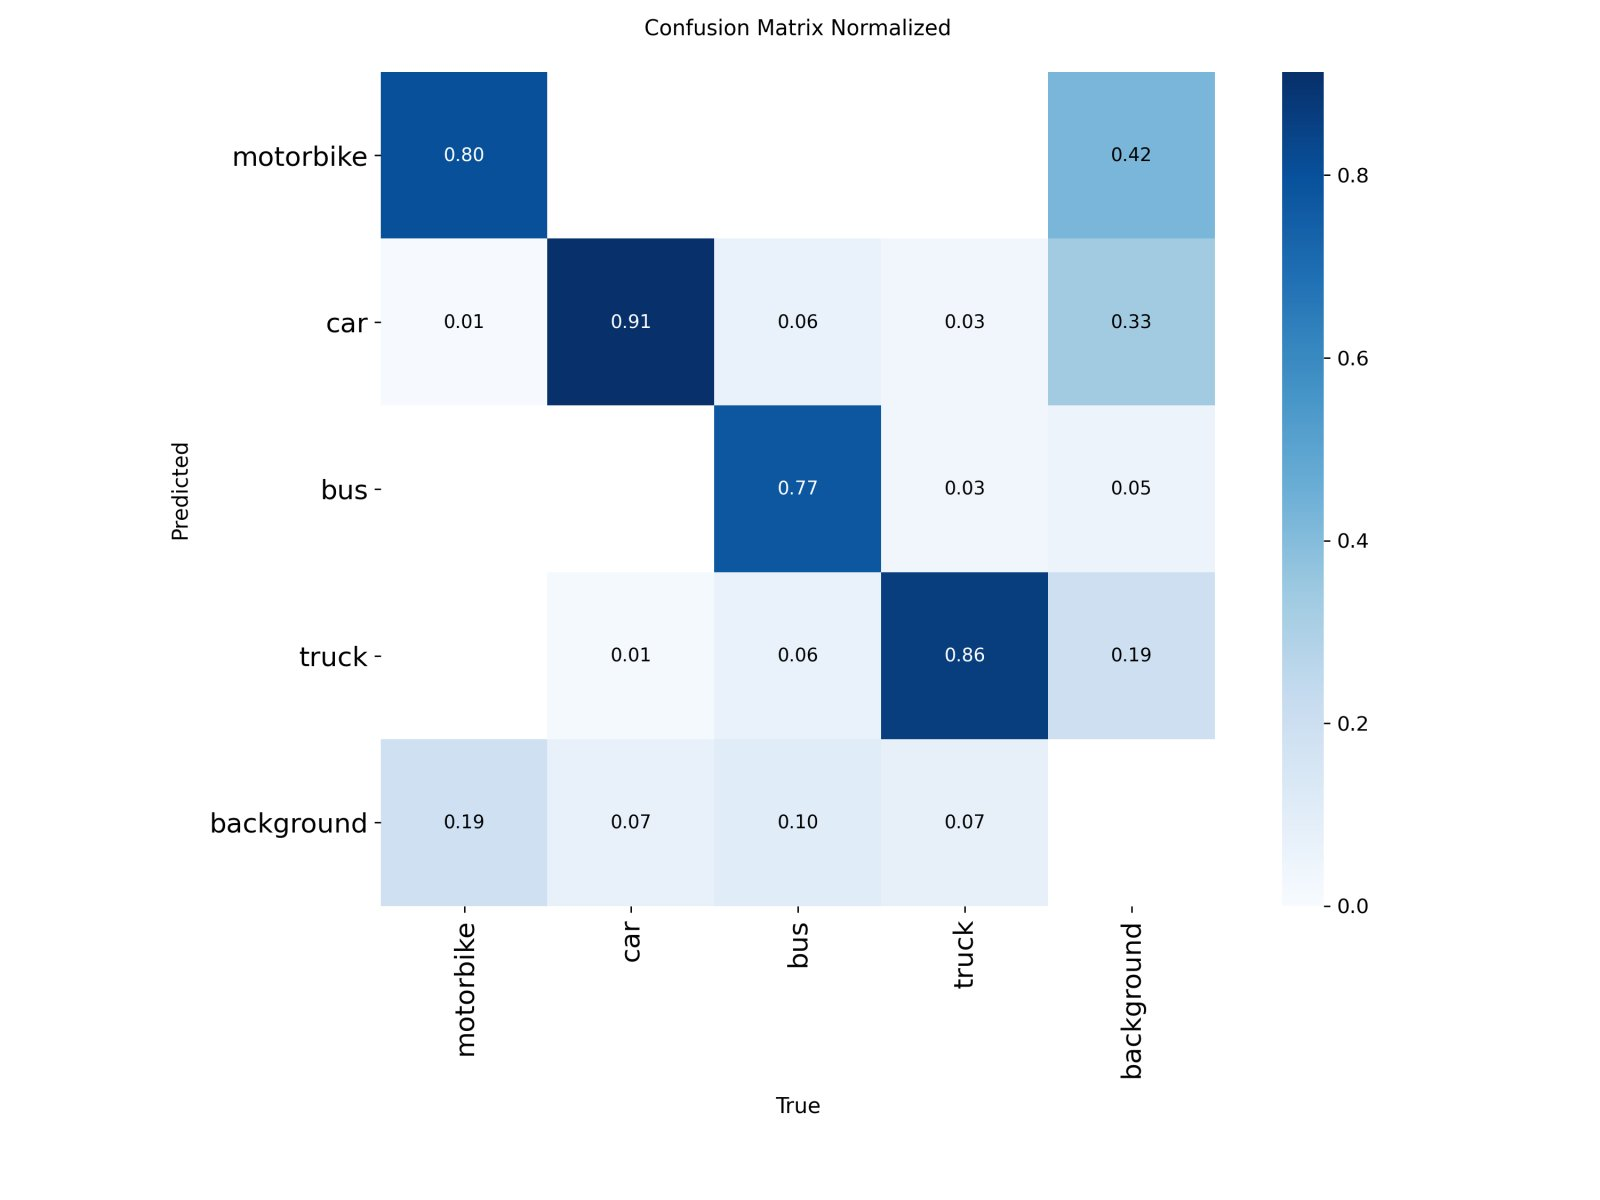
\includegraphics[width=0.72\linewidth]{v5_confusion_matrix.jpg}
  \caption{Ma trận nhầm lẫn chuẩn hoá của v5 trên tập test Roboflow (cột là lớp thật, hàng là lớp dự đoán)}
  \label{fig:confusion}
\end{figure}

\section{So sánh kiến trúc CNN và Transformer}
\label{sec:ket-qua-kien-truc}

Ba mô hình cùng dữ liệu v5, cùng giao thức (mục~\ref{sec:giao-thuc}), chấm một lần trên mọi tập.

\begin{table}[H]
  \centering
  \caption{mAP50 chính của ba kiến trúc và đối chứng cùng số điểm ảnh}
  \label{tab:kien-truc}
  \small
  \begin{tabularx}{\linewidth}{|p{3.4cm}|C|C|C|C|}
    \hline
    \thead{Tập} & \thead{YOLO26n (v5) @960} & \thead{YOLO26s @960} & \thead{RT-DETRv2-S @960×960} &
      \thead{YOLO26s @1280} \\ \hline
    Test Hà Nội & 0.923 & 0.914 & 0.929 & 0.915 \\ \hline
    \texttt{vn\_extra} ngày & 0.745 & 0.798 & \textbf{0.886} & 0.875 \\ \hline
    \texttt{vn\_extra} đêm & 0.628 & 0.713 & \textbf{0.816} & 0.800 \\ \hline
    20 frame PVD & 0.892 & 0.903 & 0.895 & 0.907 \\ \hline
    Test Roboflow (4 lớp) & 0.834 & 0.862 & 0.874 & -- \\ \hline
    Val UVH-26 (4 lớp) & 0.850 & 0.859 & \textbf{0.894} & 0.865 \\ \hline
    UA-DETRAC đêm & 0.845 & 0.876 & 0.887 & 0.862 \\ \hline
    UA-DETRAC ngày & 0.812 & 0.885 & 0.924 & 0.885 \\ \hline
  \end{tabularx}
\end{table}

\begin{table}[H]
  \centering
  \caption{mAP50-95 trên các tập có nhãn độc lập với mọi mô hình YOLO}
  \label{tab:kien-truc-5095}
  \small
  \begin{tabular}{|l|c|c|c|}
    \hline
    \thead{Tập} & \thead{YOLO26n (v5)} & \thead{YOLO26s} & \thead{RT-DETRv2-S} \\ \hline
    Val UVH-26 & 0.696 & 0.721 & \textbf{0.757} \\ \hline
    UA-DETRAC đêm & 0.538 & 0.554 & \textbf{0.588} \\ \hline
    UA-DETRAC ngày & 0.539 & 0.569 & \textbf{0.599} \\ \hline
  \end{tabular}
\end{table}

Từ Bảng~\ref{tab:kien-truc} và~\ref{tab:kien-truc-5095} rút ra ba kết luận:
\begin{enumerate}
  \item Cùng kích thước ảnh 960 (mặc định của mỗi họ), RT-DETRv2-S bằng hoặc hơn YOLO26s trên mọi tập. Chênh lệch rõ ở
        cảnh khó: \texttt{vn\_extra} ngày 0.886 so với 0.798, đêm 0.816 so với 0.713, val UVH-26 0.894 so với 0.859;
        hoà ở cảnh dễ (Hà Nội, PVD).
  \item Khi cho YOLO26s nhìn cùng số điểm ảnh (ảnh 1280), hai họ \textbf{hoà nhau} trên dữ liệu Việt Nam 1080p: khoảng tin
        cậy chồng nhau (ngày 0.875 [0.849--0.893] so với 0.886 [0.853--0.894]; đêm 0.800 [0.764--0.826] so với 0.816
        [0.782--0.840]), mAP50-95 ngày 0.588 so với 0.578, đêm 0.548 so với 0.547. Phần lớn lợi thế của RT-DETRv2 ở
        \texttt{vn\_extra} đến từ độ phân giải đầu vào chứ không phải từ kiến trúc.
  \item Trên hai tập có nhãn độc lập, RT-DETRv2-S có mAP50-95 cao hơn YOLO26s đều khoảng 0.03, tức box khít hơn. Ảnh
        UA-DETRAC chỉ 960×540 nên tăng ảnh lên 1280 không giúp YOLO (0.862 thấp hơn 0.876).
\end{enumerate}

YOLO26s hơn YOLO26n rõ ở \texttt{vn\_extra} và UA-DETRAC ngày, ngang nhau ở Hà Nội, PVD và UVH-26.
Hình~\ref{fig:acc-speed} đặt độ chính xác cạnh tốc độ CPU: mỗi bước tăng độ chính xác đều phải trả bằng thời gian xử
lý, và RT-DETRv2-S nằm xa nhất về phía chậm.

\begin{figure}[H]
  \centering
  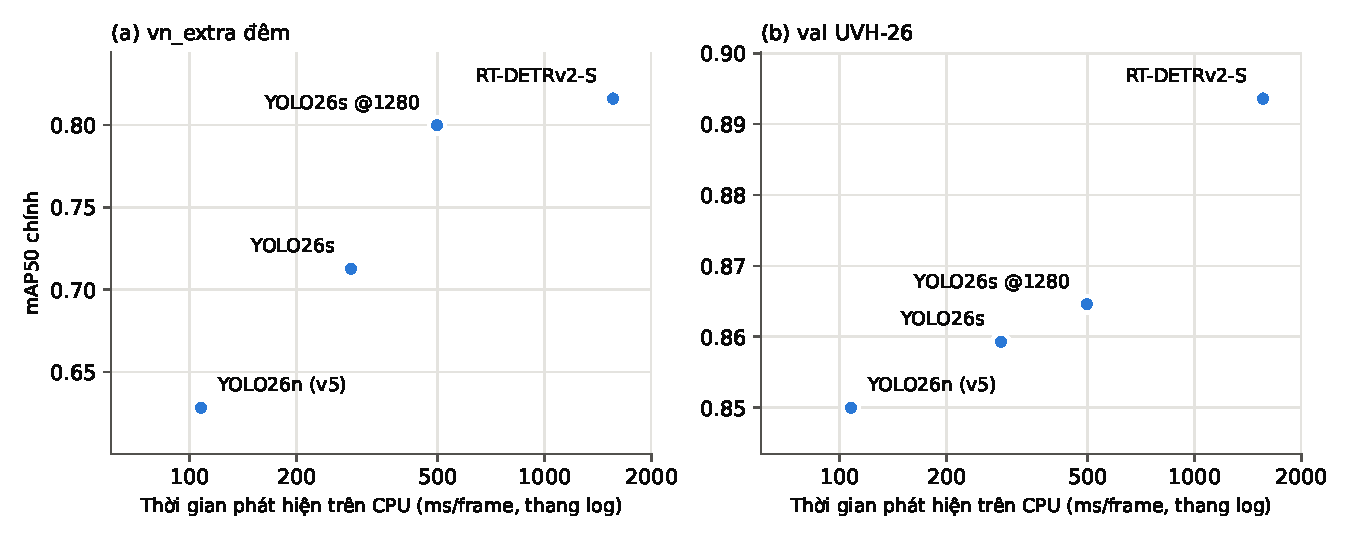
\includegraphics[width=\linewidth]{accuracy_vs_speed.pdf}
  \caption{Độ chính xác (mAP50 chính) theo thời gian phát hiện trên CPU i5-8250U của bốn cấu hình}
  \label{fig:acc-speed}
\end{figure}

\section{Tốc độ}
\label{sec:toc-do}

Laptop dòng U dễ bị hạ xung nhịp khi nóng, nên cách đo được thiết kế để công bằng giữa các mô hình: 5 đợt × 30 frame
video 1080p, các mô hình chạy xen kẽ trên cùng 30 frame và đảo thứ tự mỗi đợt, nghỉ giữa các đợt, khởi động mỗi mô hình
ít nhất 15 giây trước khi đo. ``Detector'' gồm tiền xử lý, suy luận và hậu xử lý; ``pipeline'' gồm cả đọc video và
theo dõi.

\begin{table}[H]
  \centering
  \caption{Tốc độ trên CPU Intel Core i5-8250U (ms/frame, trung vị [khoảng tứ phân vị])}
  \label{tab:toc-do-cpu}
  \footnotesize
  \begin{tabularx}{\linewidth}{|>{\raggedright\arraybackslash}p{2.2cm}|>{\centering\arraybackslash}p{1.55cm}|C|C|>{\centering\arraybackslash}p{1.15cm}|C|}
    \hline
    \thead{Mô hình} & \thead{Đầu vào} & \thead{Tham số / GFLOPs} & \thead{Detector} & \thead{frame/s} &
      \thead{Pipeline (frame/s)} \\ \hline
    YOLO26n v5, PyTorch & 544×960 & 2.51 M / 7.4 & 107.6 [92.0--129.3] & 9.3 & 206.4 (4.8) \\ \hline
    YOLO26n v5, OpenVINO & 544×960 & -- & 67.6 [64.7--74.1] & 14.8 & 155.7 (6.4) \\ \hline
    YOLO26s & 544×960 & 9.95 M / 28.7 & 284.8 [263.1--322.2] & 3.5 & 404.4 (2.5) \\ \hline
    YOLO26s @1280 & 736×1280 & 9.95 M / 52.4 & 497.3 [461.6--614.8] & 2.0 & 705.1 (1.4) \\ \hline
    RT-DETRv2-S & 960×960 & 20.08 M / 133.9 & 1561.0 [1441.7--1719.5] & 0.64 & -- \\ \hline
  \end{tabularx}
\end{table}

\begin{table}[H]
  \centering
  \caption{Tốc độ trên GPU Tesla T4 (Kaggle, PyTorch FP32; ms/frame và frame/s)}
  \label{tab:toc-do-gpu}
  \small
  \begin{tabular}{|l|c|c|}
    \hline
    \thead{Mô hình} & \thead{Detector} & \thead{Pipeline} \\ \hline
    YOLO26n v5 & 13.2 (75.7) & 23.7 (42.2) \\ \hline
    YOLO26s & 14.7 (68.0) & 23.5 (42.6) \\ \hline
    YOLO26s @1280 & 24.3 (41.2) & 33.2 (30.2) \\ \hline
    RT-DETRv2-S & 62.5 (16.0) & -- \\ \hline
  \end{tabular}
\end{table}

Trên CPU (Bảng~\ref{tab:toc-do-cpu}):
\begin{itemize}
  \item OpenVINO tăng tốc riêng phần phát hiện 1.6 lần (107.6 xuống 67.6 ms) nhưng cả pipeline chỉ 1.3 lần, vì pipeline
        còn tốn khoảng 90--100 ms mỗi frame cho giải mã video 1080p và tracker (lúc đo vẫn bật GMC). Trong một phép đo
        riêng cùng điều kiện, tắt GMC giảm thời gian pipeline OpenVINO từ 128 xuống 92 ms (7.8 lên 10.8 frame/s).
  \item RT-DETRv2-S mất 1.56 giây mỗi frame: chậm hơn YOLO26s ở ảnh 960 khoảng 5.5 lần, hơn YOLO26s ở ảnh 1280 (độ chính
        xác ngang nhau trên dữ liệu Việt Nam) 3.1 lần, hơn v5 14 lần và hơn v5 OpenVINO 23 lần. Mô hình này không dùng
        được cho video trên CPU.
\end{itemize}

Trên GPU (Bảng~\ref{tab:toc-do-gpu}), YOLO26n và YOLO26s gần như nhanh bằng nhau (cả pipeline khoảng 42 frame/s): mô
hình nhỏ không tận dụng hết GPU, phần thời gian còn lại là tiền xử lý, hậu xử lý và tracker chạy trên CPU. Vì vậy nếu có
GPU nên dùng YOLO26s, chính xác hơn ở cảnh khó mà không chậm hơn. RT-DETRv2-S trên GPU vẫn chậm hơn YOLO26s khoảng 4
lần nhưng đạt 16 frame/s cho riêng phần phát hiện.

\section{Kết quả theo dõi}
\label{sec:theo-doi}

\subsection{Tập dev VnTraffic}

\begin{table}[H]
  \centering
  \caption{So sánh ba thuật toán theo dõi trên VnTraffic (mô hình v3, tham số mặc định)}
  \label{tab:tracker}
  \small
  \begin{tabular}{|l|c|c|c|c|c|c|}
    \hline
    \thead{Tracker} & \thead{HOTA} & \thead{AssA} & \thead{IDR} & \thead{Đổi ID} & \thead{MOTA} & \thead{frame/s CPU} \\ \hline
    ByteTrack & 0.480 & 0.615 & 0.708 & 147 & 0.054 & 4.4 \\ \hline
    \textbf{BoT-SORT} & 0.505 & \textbf{0.659} & \textbf{0.738} & \textbf{128} & 0.068 & 3.6 \\ \hline
    OC-SORT & 0.493 & 0.594 & 0.669 & 206 & 0.227 & 4.0 \\ \hline
  \end{tabular}
\end{table}

BoT-SORT tốt nhất trên cả ba chỉ số không phụ thuộc phát hiện thừa (Bảng~\ref{tab:tracker}). MOTA ở đây rất thấp và
không dùng để kết luận: khoảng 21 box mỗi frame của tracker không khớp nhãn, phần lớn là xe máy thật trong cụm dày mà
nhãn bỏ sót. OC-SORT có MOTA cao hơn chỉ vì xuất ít box hơn.

Chỉnh lưới 18 cấu hình BoT-SORT và ByteTrack: giữ track mất 90 frame, không ReID cho IDR 0.744 và AssA 0.668 (mặc định:
0.738 và 0.659), số lần đổi ID không đổi (128). Bật ReID làm số lần đổi ID tăng lên 207--211. Lọc track dưới 3 frame giảm
đổi ID từ 128 xuống 118, IDR giảm 0.004.

\begin{table}[H]
  \centering
  \caption{Ảnh hưởng của mô hình phát hiện lên theo dõi trên VnTraffic (cùng BoT-SORT đã chỉnh)}
  \label{tab:detector-tracking}
  \small
  \begin{tabular}{|l|c|c|c|c|c|c|}
    \hline
    \thead{Detector} & \thead{HOTA} & \thead{AssA} & \thead{IDR} & \thead{Đổi ID} & \thead{FN} & \thead{Số track} \\ \hline
    v3 & 0.507 & 0.668 & 0.744 & 128 & 2.550 & 467 \\ \hline
    v4 @1280 & 0.555 & 0.684 & 0.738 & 91 & 2.697 & 344 \\ \hline
    \textbf{v5} & 0.554 & \textbf{0.709} & \textbf{0.827} & \textbf{62} & \textbf{1.058} & 334 \\ \hline
    v5 @1280 & 0.549 & 0.713 & 0.820 & 85 & 1.183 & 341 \\ \hline
  \end{tabular}
\end{table}

Đổi từ v3 sang v5 là cải tiến lớn nhất cho theo dõi (Bảng~\ref{tab:detector-tracking}): số box bỏ sót giảm hơn một nửa
(2.550 xuống 1.058), IDR tăng từ 0.744 lên 0.827, số lần đổi ID giảm từ 128 xuống 62. Soi từng xe, các xe v3 bỏ sót
như một xe buýt (điểm tin cậy 0 lên 0.84--0.87 với v5), một xe tải (dưới 0.14 lên 0.93--0.94) và một xe máy đang dừng
(0.01--0.12 lên 0.52--0.82) đều được v5 nhận ra. Phát hiện ổn định thì quỹ đạo ít bị đứt. Tắt GMC cho kết quả gần như
y hệt (IDR 0.827 cả hai bản, đổi ID 61 so với 62).

\subsection{Tập test clip Phạm Văn Đồng}

\begin{table}[H]
  \centering
  \caption{Kết quả theo dõi trên tập test (clip Phạm Văn Đồng 20 giây, 183 quỹ đạo nhãn)}
  \label{tab:tracking-test}
  \footnotesize
  \begin{tabularx}{\linewidth}{|L|c|c|c|c|c|c|c|c|}
    \hline
    \thead{Cấu hình} & \thead{HOTA} & \thead{DetA} & \thead{AssA} & \thead{MOTA} & \thead{IDF1} & \thead{IDR} & \thead{IDP} &
      \thead{Đổi ID} \\ \hline
    v5 + BoT-SORT đã chỉnh, không GMC (mặc định) & 0.718 & 0.670 & 0.784 & 0.813 & 0.880 & 0.822 & 0.947 & 26 \\ \hline
    v5 + BoT-SORT đã chỉnh, có GMC & 0.718 & 0.672 & 0.783 & 0.815 & 0.880 & 0.822 & 0.946 & 28 \\ \hline
  \end{tabularx}
\end{table}

Trên tập test có nhãn đầy đủ, cấu hình mặc định đạt HOTA 0.718, MOTA 0.813, IDF1 0.880, đổi ID 26 lần trên 183 xe
(Bảng~\ref{tab:tracking-test}). IDP 0.947 cao hơn IDR 0.822: hệ thống ít khi gán nhầm danh tính, phần mất chủ yếu
do bỏ sót (2.157 box bỏ sót so với 357 box thừa).

\begin{table}[H]
  \centering
  \caption{Ablation trên tập test (chỉ để báo cáo, lựa chọn đã chốt trên dev)}
  \label{tab:ablation}
  \small
  \begin{tabular}{|l|c|c|c|c|}
    \hline
    \thead{Detector + tracker} & \thead{HOTA} & \thead{MOTA} & \thead{IDF1} & \thead{Đổi ID} \\ \hline
    v5 + BoT-SORT & 0.718 & 0.815 & 0.880 & 28 \\ \hline
    v5 + ByteTrack & 0.698 & 0.791 & 0.872 & 34 \\ \hline
    v5 + OC-SORT & 0.692 & 0.786 & 0.865 & 56 \\ \hline
    v3 + BoT-SORT đã chỉnh & 0.741 & 0.763 & 0.845 & 44 \\ \hline
  \end{tabular}
\end{table}

Bảng~\ref{tab:ablation} xác nhận lựa chọn trên dev: với cùng v5, BoT-SORT tốt nhất trên test. So v5 với v3, v5 hơn rõ ở
MOTA (0.815 so với 0.763), IDF1 (0.880 so với 0.845) và số lần đổi ID (28 so với 44). HOTA trung bình của v3 cao hơn
(0.741 so với 0.718) nhưng đây là thiên lệch do nhãn sơ bộ, phân tích ở mục~\ref{sec:thao-luan}. Lọc track dưới 3 frame
giảm đổi ID của v5 từ 28 xuống 23, HOTA giảm nhẹ từ 0.718 xuống 0.708.

\section{Sai số đếm xe qua vạch}
\label{sec:dem-xe}

Số lượt xe thật được tính bằng cách cho các quỹ đạo nhãn tay của clip test đi qua đúng bộ đếm của hệ thống, nên chênh
lệch chỉ do phát hiện và theo dõi. Vạch đếm là vạch mặc định của hệ thống (nằm ngang ở 60\% chiều cao ảnh), không chọn
theo kết quả.

\begin{table}[H]
  \centering
  \caption{Số lượt xe qua vạch trên clip test 20 giây: nhãn tay và hệ thống}
  \label{tab:dem-xe}
  \small
  \begin{tabular}{|l|c|c|c|c|c|c|c|}
    \hline
    \thead{Lớp} & \thead{Thật vào} & \thead{Thật ra} & \thead{Đếm vào} & \thead{Đếm ra} & \thead{Thật tổng} &
      \thead{Đếm tổng} & \thead{Sai số} \\ \hline
    Xe máy & 1 & 52 & 0 & 53 & 53 & 53 & 2 \\ \hline
    Ô tô & 1 & 18 & 0 & 19 & 19 & 19 & 2 \\ \hline
    Xe buýt & 0 & 1 & 0 & 0 & 1 & 0 & 1 \\ \hline
    Xe tải & 0 & 0 & 0 & 0 & 0 & 0 & 0 \\ \hline
    \textbf{Tổng} & 2 & 71 & 0 & 72 & 73 & 72 & 3 (4.1\%) \\ \hline
  \end{tabular}
\end{table}

Hệ thống đếm 72 lượt so với 73 lượt thật (Bảng~\ref{tab:dem-xe}); tổng theo lớp khớp hoàn toàn ở xe máy (53) và ô tô
(19). Sai số tính theo từng hướng là 3 lượt. Xem lại từng lượt:
\begin{itemize}
  \item Hai lượt ``vào'' của nhãn (một ô tô, một xe máy) là hiện tượng của nhãn ở tán cây: xe khuất dần sau cây, box nhãn
        chỉ ôm phần nhìn thấy nên cạnh đáy box đi ngược lên qua vạch, dù xe không đi ngược chiều. Vạch y = 0.6 đi qua mép
        tán cây bên phải.
  \item Lượt xe buýt là một chiếc Ford Transit bị đếm thành ô tô, đúng vấn đề định nghĩa lớp van đã nêu.
\end{itemize}

Như vậy lỗi thật của hệ thống trên clip này là 1 lượt sai lớp; không có xe bị sót hay bị đếm trùng. Khi triển khai, nên
đặt vạch đếm ở vùng không bị che.

\section{Kết quả ở cảnh ban đêm}

Ba nguồn bằng chứng về cảnh đêm cho cùng một hướng:
\begin{itemize}
  \item \textbf{\texttt{vn\_extra} đêm} (cảnh đêm Việt Nam có nhãn): v5 đạt 0.628, cao hơn v3 (0.437) và mô hình gốc
        COCO (0.437); YOLO26s đạt 0.713, RT-DETRv2-S 0.816.
  \item \textbf{UA-DETRAC}: cả ba mô hình COCO, v3, v5 không giảm độ chính xác khi trời tối (v5: đêm 0.845, ngày
        0.812). Tuy vậy đêm của UA-DETRAC là đường phố có đèn, chủ yếu ô tô, khác đường tối ở hầm chui.
  \item \textbf{Ba clip hầm chui không có nhãn}, dùng chỉ số thay thế trên 20 giây mỗi clip với mốc ban ngày là clip
        Phạm Văn Đồng: độ tin cậy trung vị của v5 là 0.59--0.63 ban đêm so với 0.63 ban ngày, tỉ lệ track ngắn dưới 1
        giây 47--52\% so với 54\%, tức v5 gần như không suy giảm; v3 tụt rõ (độ tin cậy 0.36--0.45, 67--73\% track
        ngắn). Đây là chỉ số thay thế, chỉ dùng để so tương đối.
\end{itemize}

\section{Phân tích lỗi}
\label{sec:phan-tich-loi}

Các ảnh dưới đây được chọn bằng cách đếm lỗi của v5 (ngưỡng tin cậy 0.25, ghép IoU 0.5) trên các tập test và lấy ảnh có
nhiều lỗi loại đó nhất. Màu box: xanh lá là đúng, đỏ là bỏ sót, cam là sai lớp, tím là thừa, xám là vùng bỏ qua. Ảnh chỉ
để minh hoạ; số lượng lỗi định lượng nằm ở các bảng phía trên.

\begin{figure}[H]
  \centering
  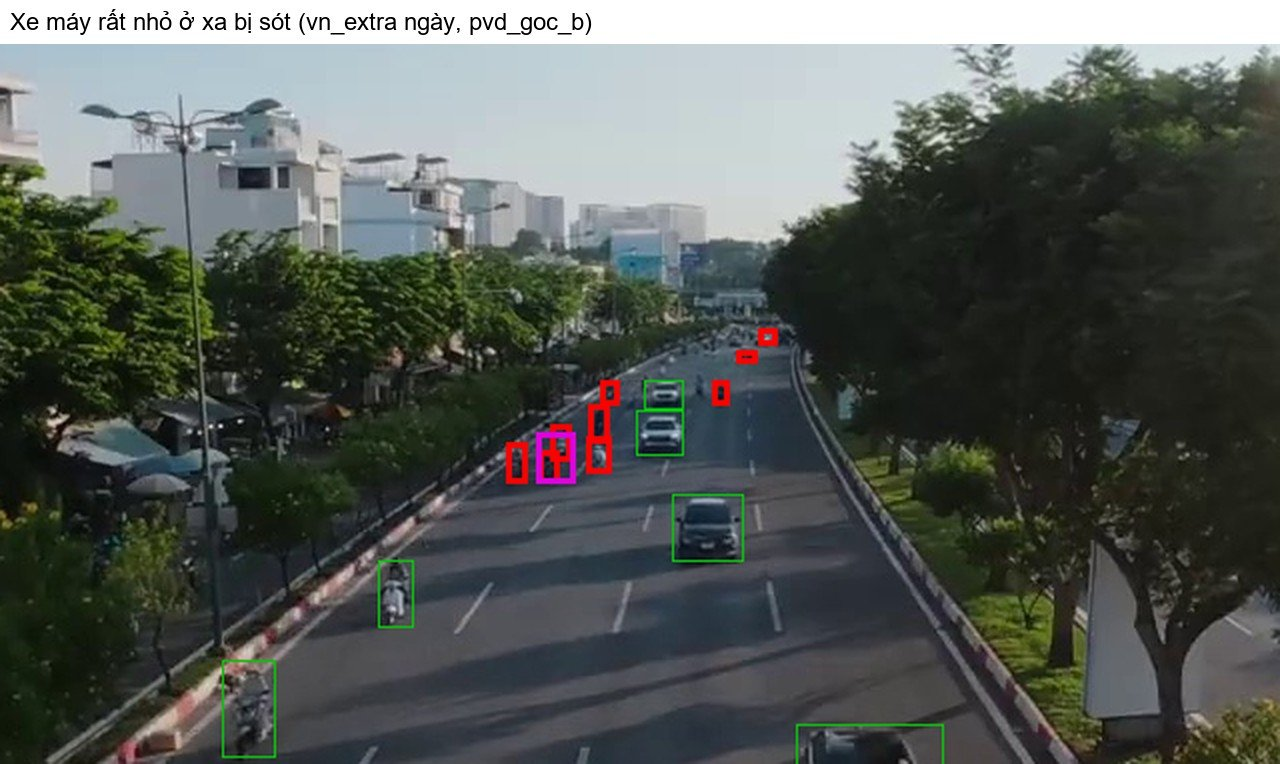
\includegraphics[width=0.9\linewidth]{error_1.jpg}
  \caption{Lỗi 1: xe máy rất nhỏ ở xa bị bỏ sót (\texttt{vn\_extra} ngày, góc máy B)}
  \label{fig:error-1}
\end{figure}

\begin{figure}[H]
  \centering
  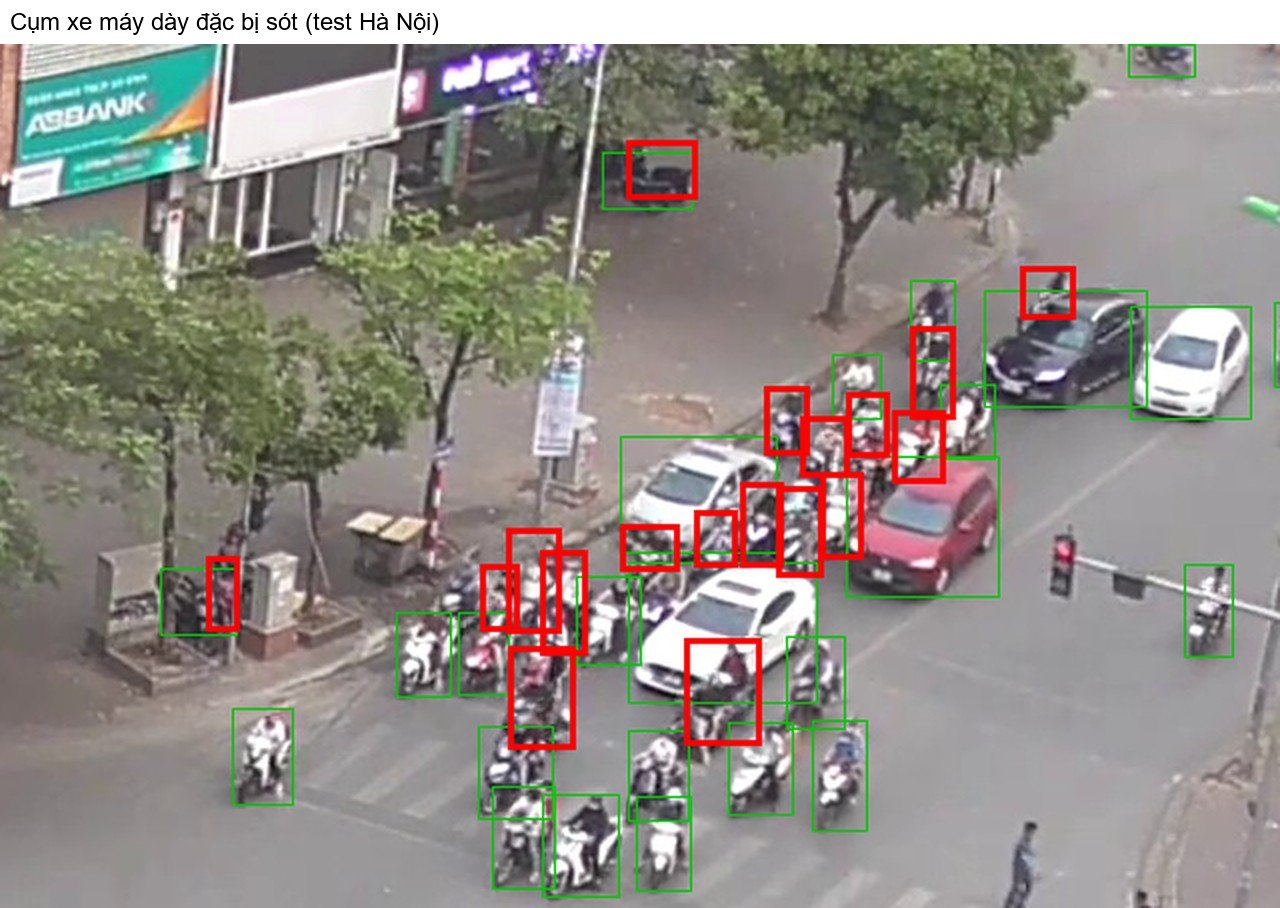
\includegraphics[width=0.9\linewidth]{error_2.jpg}
  \caption{Lỗi 2: cụm xe máy chờ đèn đỏ dày đặc bị bỏ sót (test Hà Nội)}
  \label{fig:error-2}
\end{figure}

Lỗi 1 và 2 (Hình~\ref{fig:error-1}, \ref{fig:error-2}) là hai dạng bỏ sót chính ban ngày: xe quá nhỏ sau khi ảnh bị thu
về 960 điểm ảnh, và xe máy dừng sát nhau che khuất lẫn nhau.

\begin{figure}[H]
  \centering
  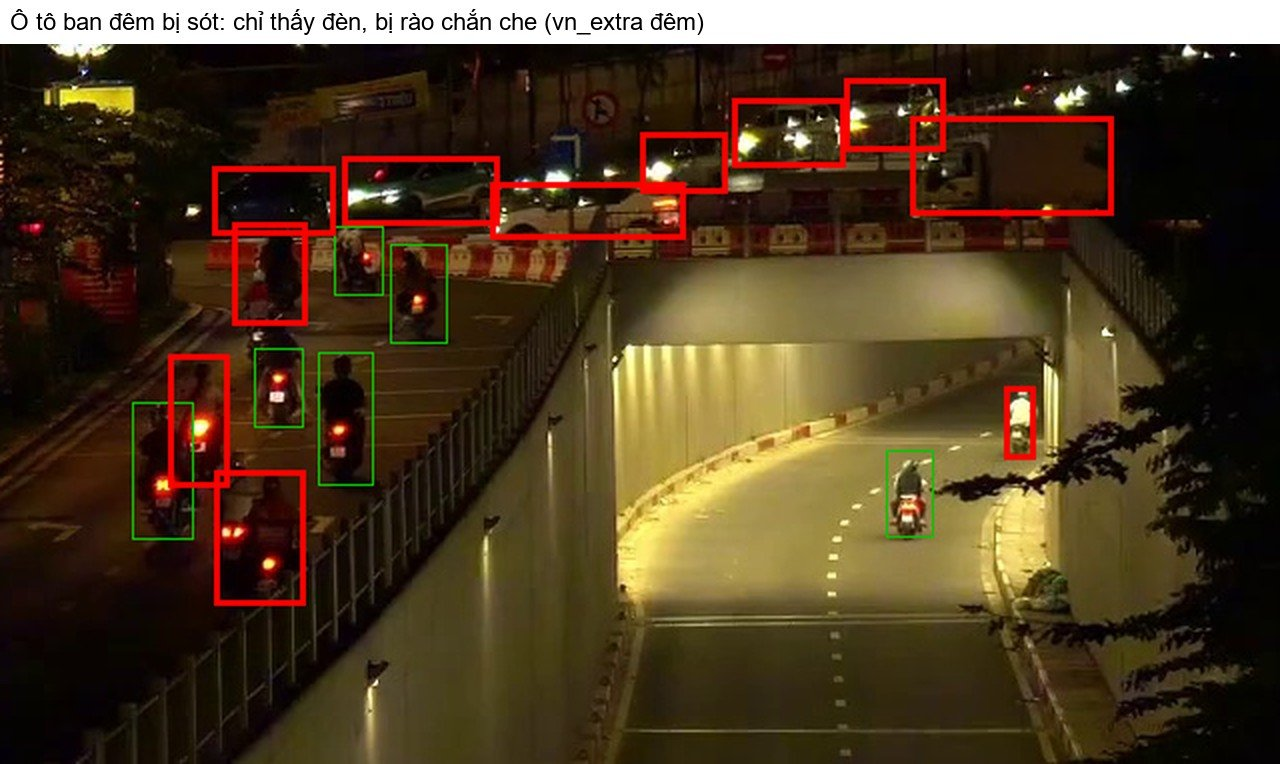
\includegraphics[width=0.9\linewidth]{error_3.jpg}
  \caption{Lỗi 3: ô tô ban đêm ở đường ngang phía xa bị rào chắn che, chỉ thấy đèn (\texttt{vn\_extra} đêm)}
  \label{fig:error-3}
\end{figure}

\begin{figure}[H]
  \centering
  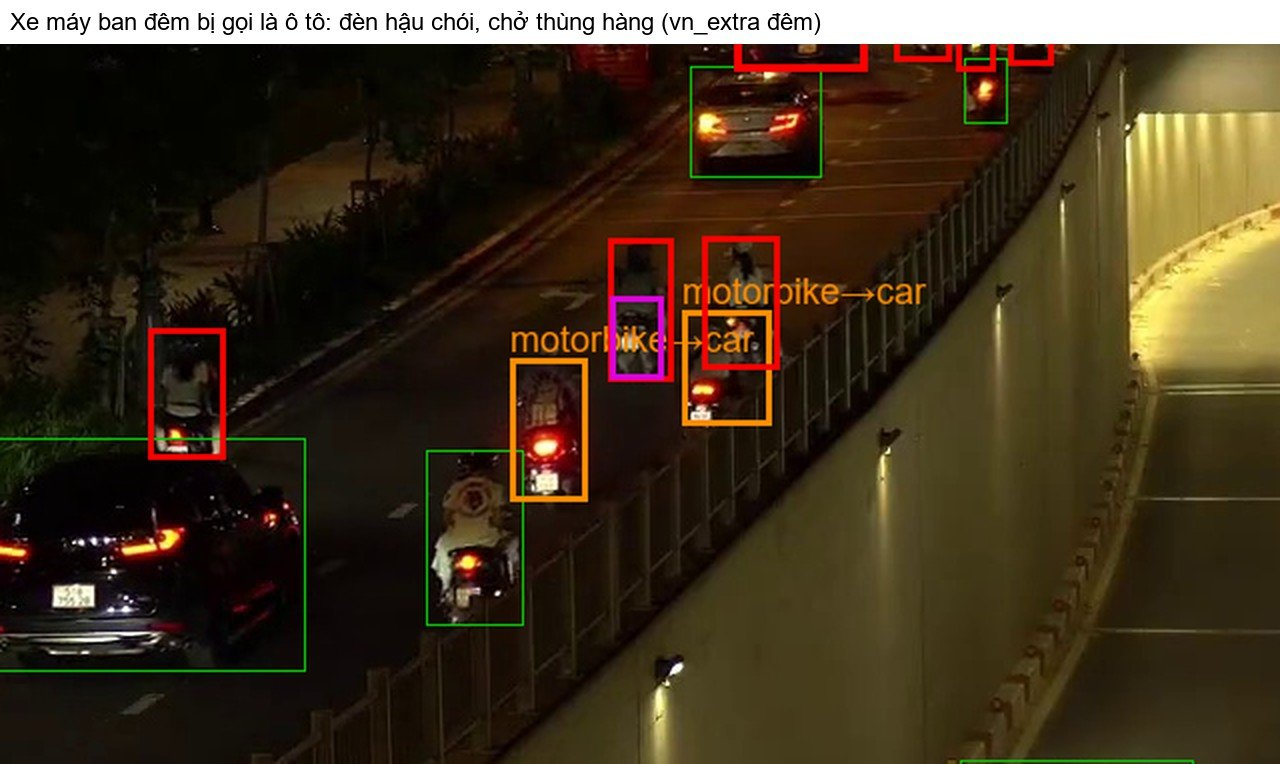
\includegraphics[width=0.9\linewidth]{error_4.jpg}
  \caption{Lỗi 4: xe máy ban đêm bị gọi là ô tô do đèn hậu chói, xe chở thùng hàng (\texttt{vn\_extra} đêm)}
  \label{fig:error-4}
\end{figure}

\begin{figure}[H]
  \centering
  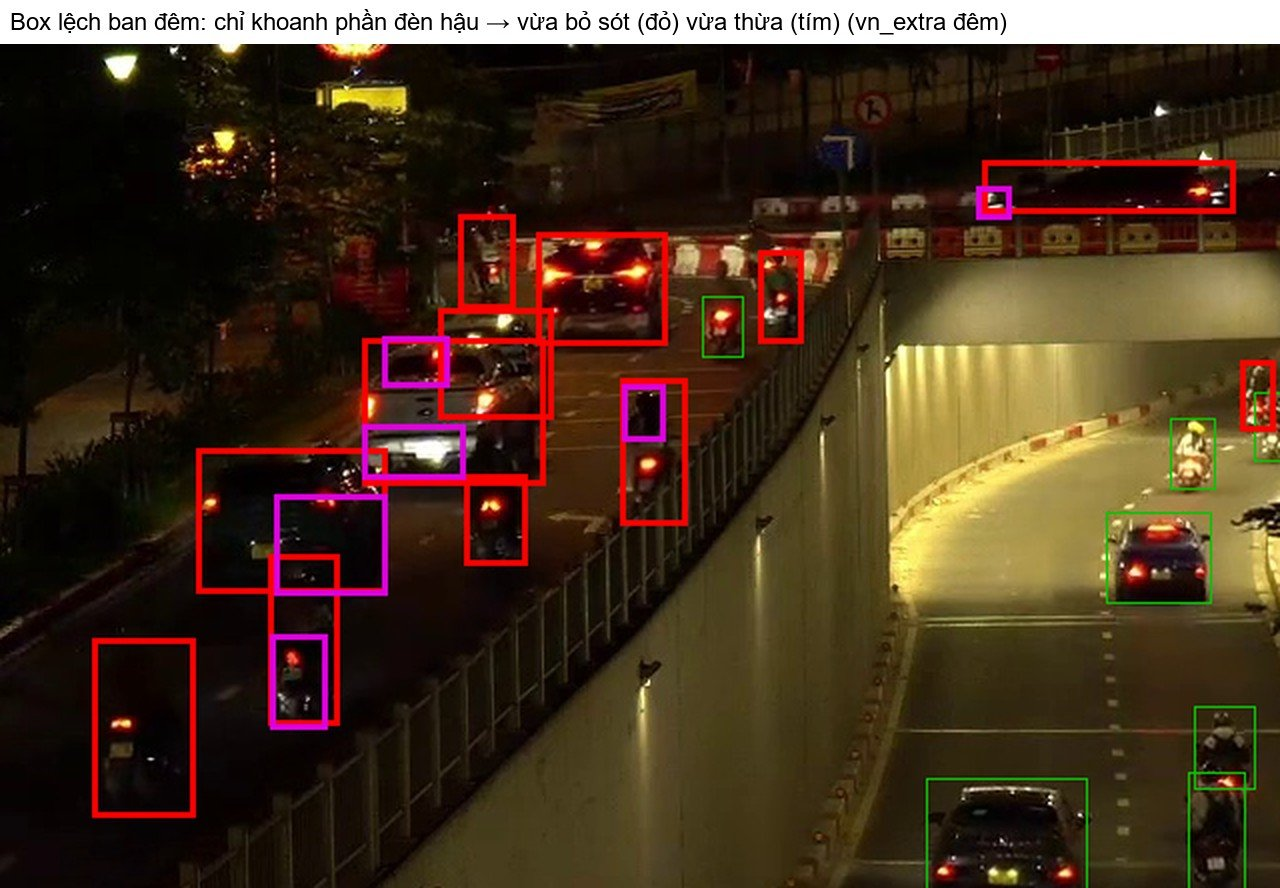
\includegraphics[width=0.9\linewidth]{error_5.jpg}
  \caption{Lỗi 5: box lệch ban đêm, mô hình chỉ khoanh phần đèn hậu sáng nên một xe bị tính cả bỏ sót (đỏ) lẫn thừa
           (tím) (\texttt{vn\_extra} đêm)}
  \label{fig:error-5}
\end{figure}

Ở cảnh đêm (Hình~\ref{fig:error-3}--\ref{fig:error-5}), ngoài xe chỉ thấy đèn bị sót, có hai lỗi đặc trưng. Xe máy chở
hàng có đèn chói bị gọi là ô tô. Và mô hình hay chỉ khoanh phần đèn hậu sáng: box này có IoU dưới 0.5 với box nhãn (bao
cả người và xe), nên một xe vừa bị tính là bỏ sót vừa sinh một phát hiện thừa. Phần lớn ``phát hiện thừa'' ban đêm thuộc
loại này chứ không phải vệt đèn hay bóng phản chiếu.

\begin{figure}[H]
  \centering
  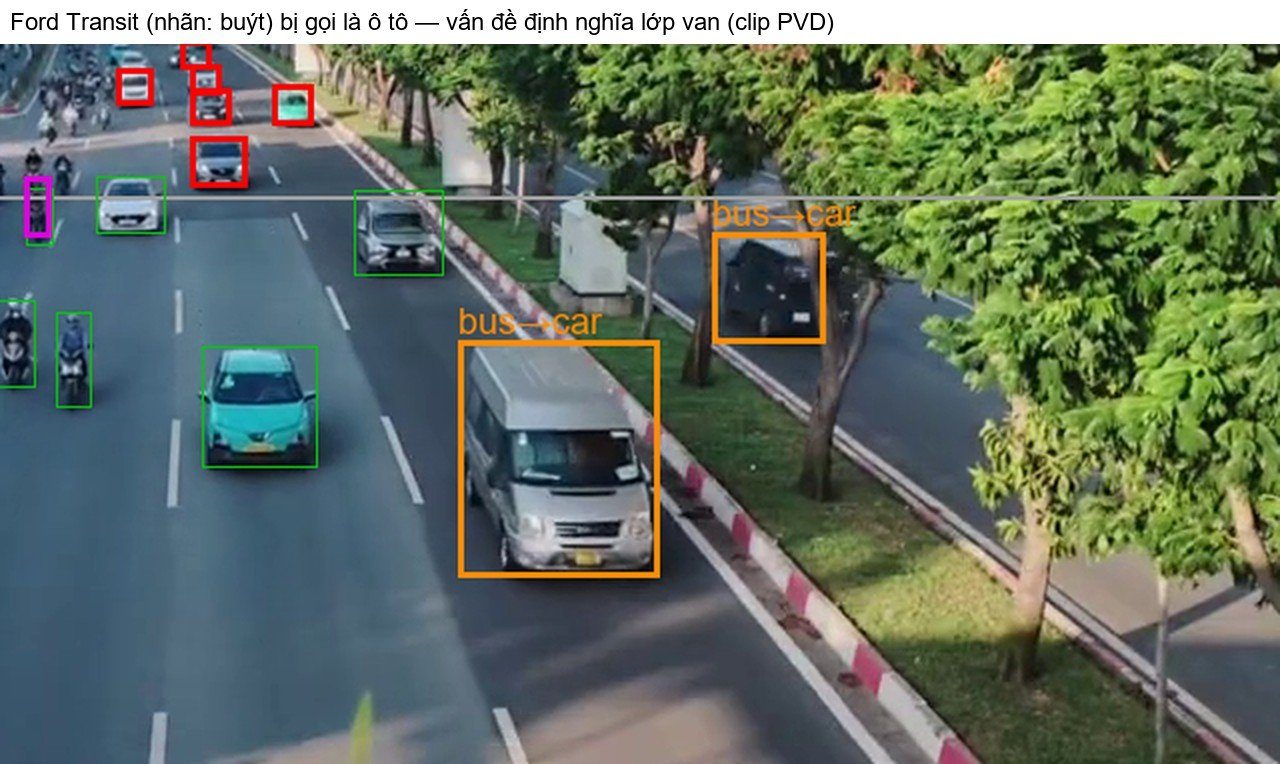
\includegraphics[width=0.9\linewidth]{error_6.jpg}
  \caption{Lỗi 6: xe Ford Transit (nhãn xe buýt) bị gọi là ô tô (clip Phạm Văn Đồng)}
  \label{fig:error-6}
\end{figure}

\begin{figure}[H]
  \centering
  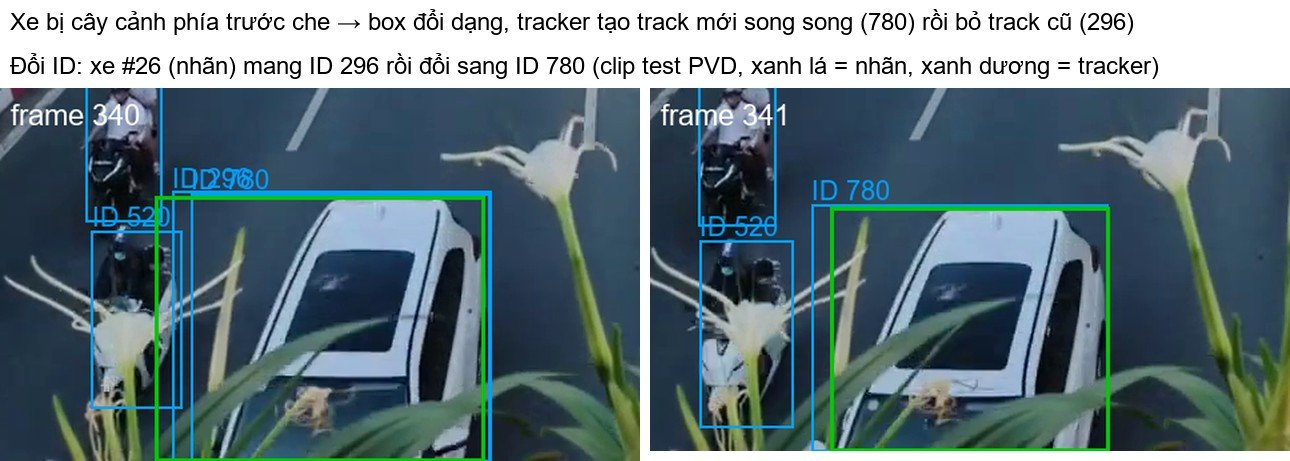
\includegraphics[width=\linewidth]{error_7.jpg}
  \caption{Lỗi 7: đổi ID khi xe bị cây cảnh phía trước che; box đổi dạng, tracker tạo track mới song song rồi bỏ track
           cũ (clip Phạm Văn Đồng)}
  \label{fig:error-7}
\end{figure}

Lỗi 6 (Hình~\ref{fig:error-6}) là hệ quả của định nghĩa lớp xe van. Lỗi 7 (Hình~\ref{fig:error-7}) là dạng đổi ID điển
hình: khi xe đi sau cây, box co lại theo phần nhìn thấy, tracker không ghép được với track cũ nên tạo track mới. Bộ dò
đổi ID đơn giản của đề tài (ghép IoU từng frame) đếm được 46 lần; lọc thêm điều kiện ``ID cũ đã biến mất ở frame đổi''
còn 25 lần, gần với 26 lần đổi ID của TrackEval. Phần chênh lệch là box của tracker nhảy qua lại giữa hai track trùng
trên cùng một xe.

\section{Ứng dụng web và video demo}

Web demo (Hình~\ref{fig:app}) cho chọn clip, xem video kết quả có box, ID, vết di chuyển và vạch đếm, cùng bảng đếm
theo lớp và hướng, biểu đồ số xe cộng dồn theo thời gian, danh sách sự kiện và nút tải CSV. Chế độ mặc định nạp video
đã xử lý sẵn trên GPU để trình chiếu mượt; chế độ chạy trực tiếp trên CPU dùng khi cần xử lý video mới.

\begin{figure}[H]
  \centering
  \begin{subfigure}{\linewidth}
    \centering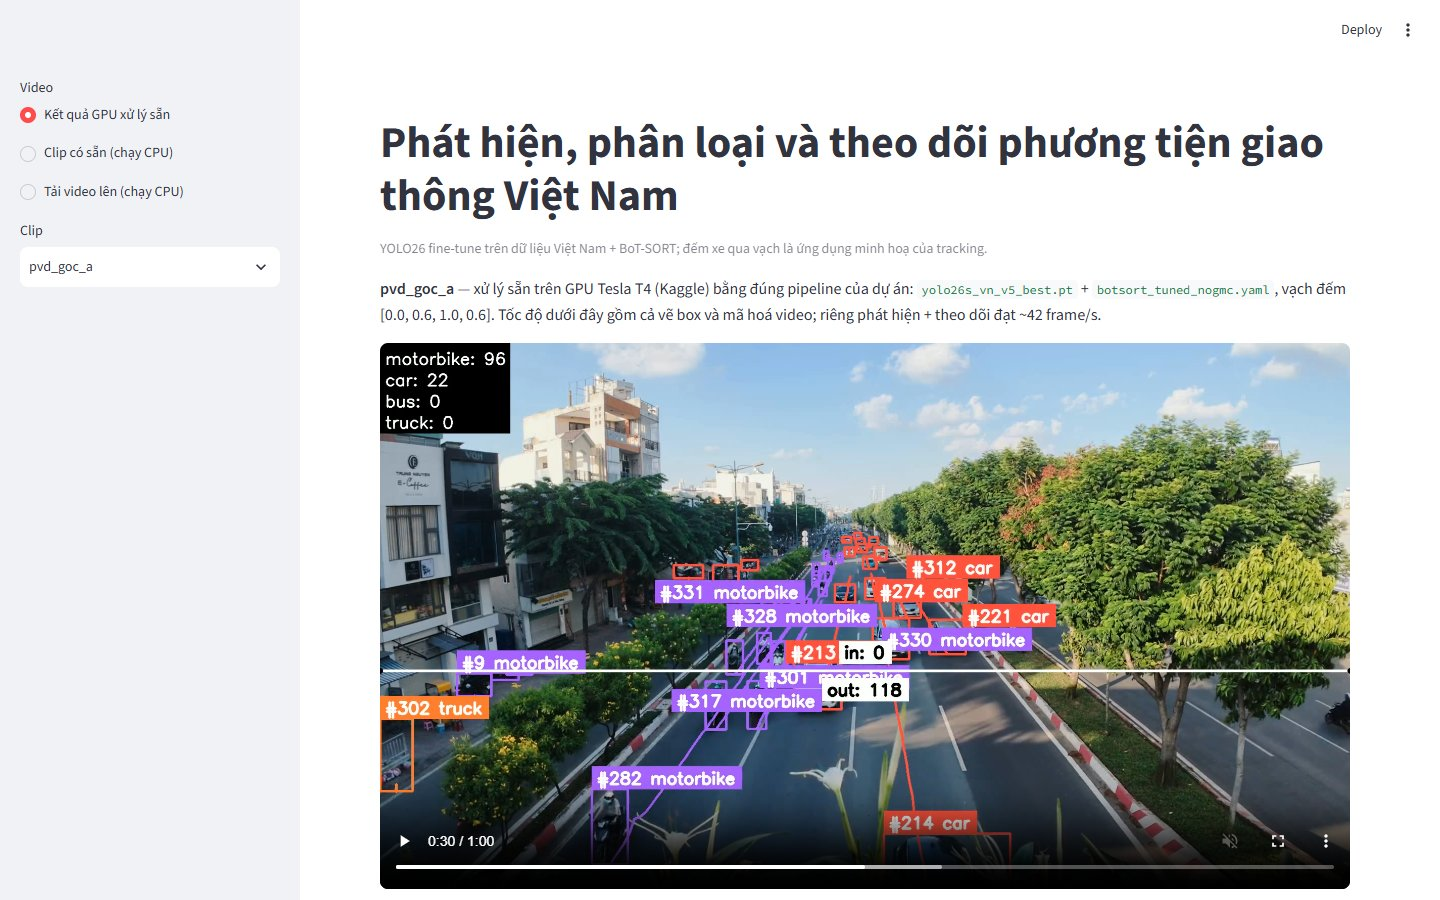
\includegraphics[width=0.92\linewidth]{app_gpu_demo.jpg}
    \caption{Video kết quả của clip Phạm Văn Đồng}
  \end{subfigure}\\[6pt]
  \begin{subfigure}{\linewidth}
    \centering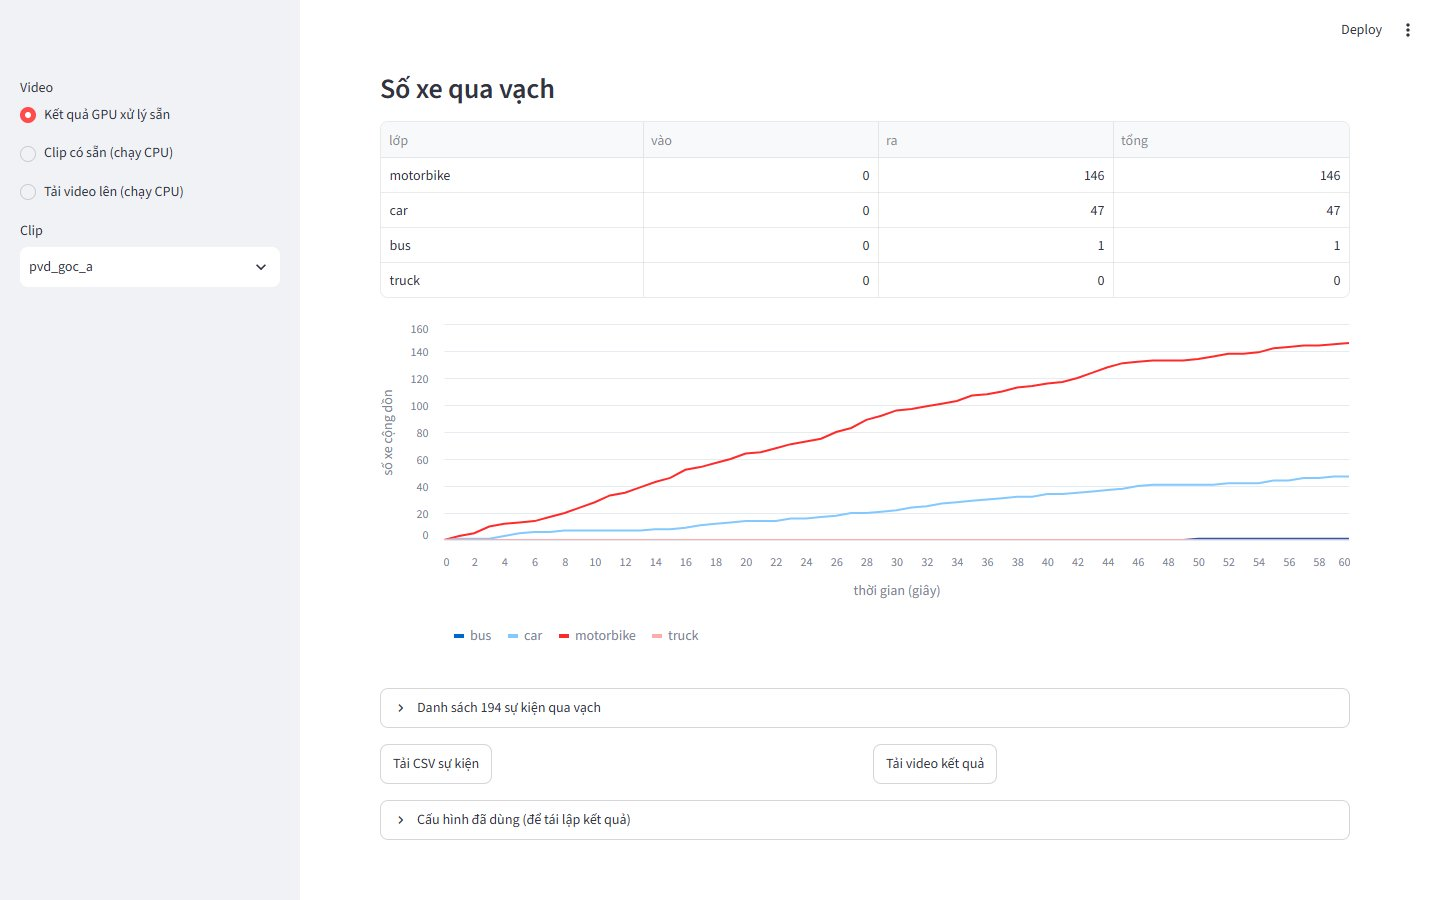
\includegraphics[width=0.92\linewidth]{app_counts.jpg}
    \caption{Bảng đếm theo lớp và hướng, biểu đồ số xe cộng dồn}
  \end{subfigure}
  \caption{Giao diện web demo Streamlit}
  \label{fig:app}
\end{figure}

Sáu clip demo dài 60 giây (ba góc máy đại lộ Phạm Văn Đồng và ba đoạn hầm chui ban đêm) được xử lý sẵn trên GPU T4 bằng
YOLO26s ở ảnh 960 và BoT-SORT đã chỉnh, đúng chương trình dùng trên máy local. Tính cả vẽ kết quả và mã hoá video 1080p,
tốc độ xử lý là 15.4--20.9 frame/s; con số này thấp hơn khoảng 42 frame/s của riêng phát hiện và theo dõi, vì khi có
GPU thì việc vẽ và ghi video trên CPU trở thành phần chậm nhất. Số lượt qua vạch trong 60 giây: góc A 194 (chỉ chiều ra,
vì làn ngược chiều ra khỏi khung hình trước vạch), góc B 169, góc C 254; ba đoạn hầm chui 69, 76 và 98. Các clip này
chưa có nhãn nên những con số này không phải số đánh giá. Hình~\ref{fig:demo-dem} là một frame của clip ban đêm.

\begin{figure}[H]
  \centering
  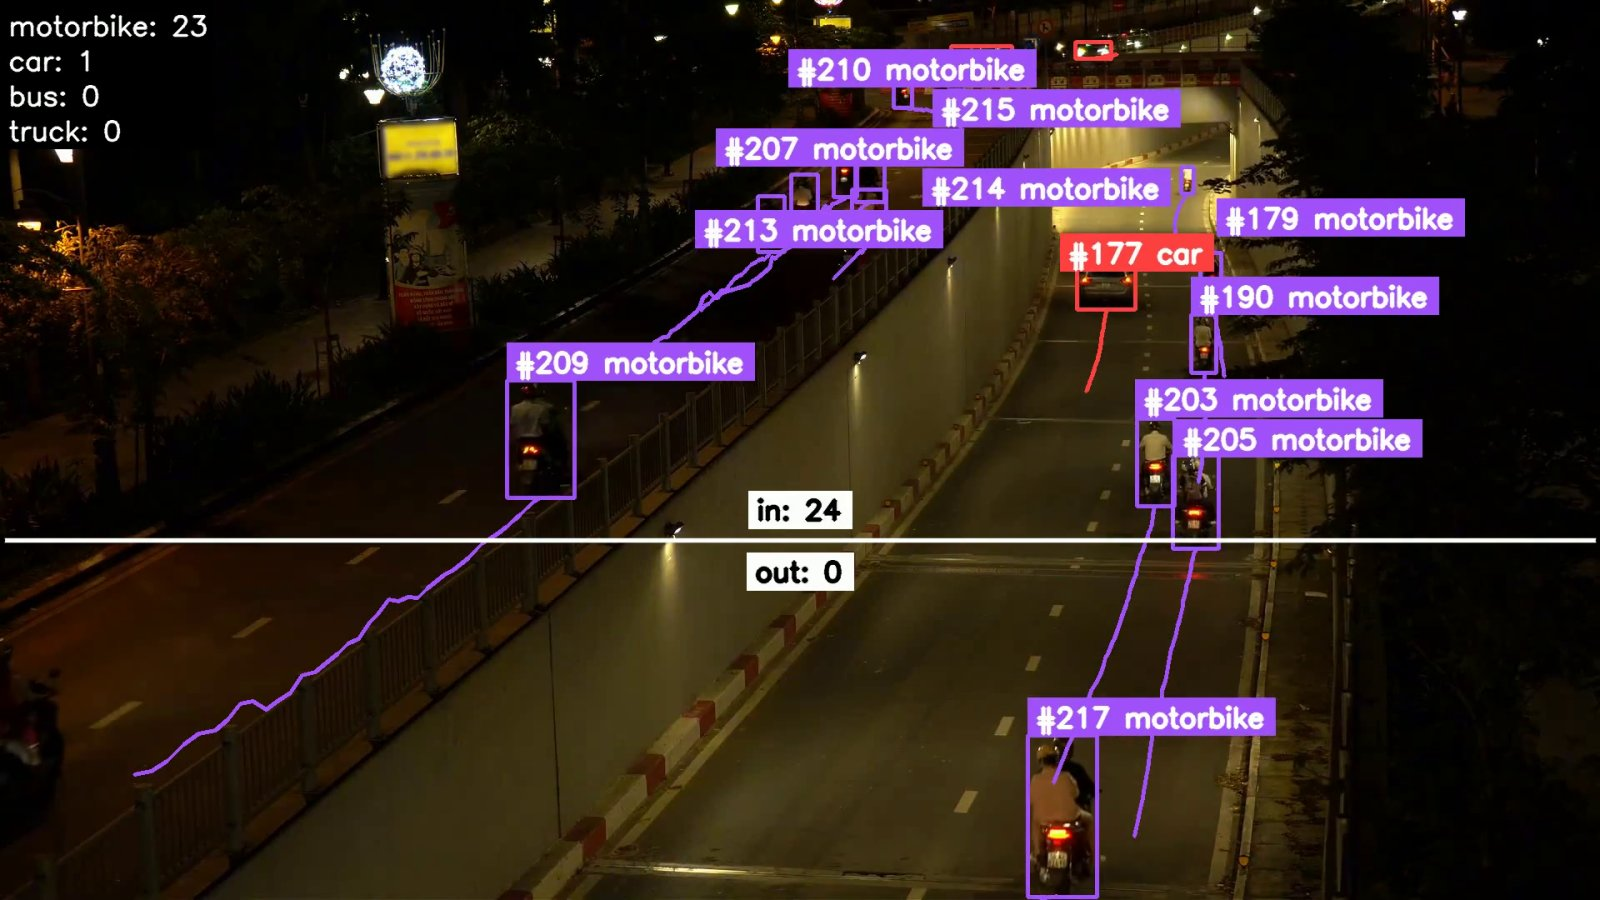
\includegraphics[width=0.92\linewidth]{demo_ham_chui_dem_1.jpg}
  \caption{Frame video demo ban đêm ở lối vào hầm chui TP.HCM (nguồn video: kênh YouTube Midnight Soundscape)}
  \label{fig:demo-dem}
\end{figure}

\section{Nhận xét và thảo luận}
\label{sec:thao-luan}

\textbf{Thiên lệch do nhãn sơ bộ.} Nhãn tay của đề tài đều được sửa từ nhãn sơ bộ của một mô hình, và box người gán giữ
nguyên mang cách khoanh box của mô hình đó. Ở test Hà Nội, 69\% box là box sơ bộ của v2 giữ nguyên, nên mAP50-95 thiên vị
mạnh v2: v2 đạt 0.815 trong khi v3 chỉ 0.765, ngược với mọi chỉ số khác. Clip Phạm Văn Đồng có nhãn sơ bộ từ v3, nên
HOTA của v3 cao hơn v5 chỉ ở các ngưỡng IoU chặt: ở IoU 0.5 HOTA của v5 là 0.844 so với 0.825 của v3, còn ở IoU 0.9 là
0.295 so với 0.412. Trên test Hà Nội (nhãn sơ bộ từ v2, không phải v3), mAP50-95 của v5 và v3 bằng nhau. Vì vậy trên các
tập này đề tài chỉ dùng mAP50 và các chỉ số theo dõi ở ngưỡng mặc định; so box khít (mAP50-95) chỉ trên tập có nhãn độc
lập. Tập \texttt{vn\_extra} được làm sau khi nhận ra vấn đề này, với nhãn sơ bộ từ một mô hình không tham gia so sánh.

\textbf{Vì sao chọn v5 và BoT-SORT.} Trên tập phát hiện Hà Nội, v3, v4, v5 hoà nhau; v5 được chọn vì tác động lên theo
dõi (đổi ID giảm một nửa trên dev) và vì tốt hơn rõ ở cảnh đêm, UVH-26 và UA-DETRAC. Điều này cho thấy dữ liệu đúng góc
camera giao thông quan trọng hơn kích thước ảnh: v4 (ảnh 1280) chỉ sửa được 1/4 số frame xe máy từng bị sót, còn v5 ở
ảnh 960 nhận ra được phần lớn các trường hợp đó. Ngoại lệ là cảnh có nhiều xe rất nhỏ ở xa, nơi ảnh 1280 có lợi rõ.

\textbf{Đánh đổi độ chính xác và tốc độ.} RT-DETRv2-S chính xác nhất và cho box khít nhất, nhưng chậm 23 lần so với v5
OpenVINO trên CPU. Khi cho YOLO cùng số điểm ảnh, khoảng cách độ chính xác trên dữ liệu Việt Nam gần như biến mất. Vì vậy
mô hình triển khai là v5 (OpenVINO) trên CPU; nếu có GPU thì dùng YOLO26s; RT-DETRv2-S là mức trần độ chính xác để tham
chiếu.

\section{Kết luận chương}

\subsection{Những kết quả chính}

\begin{itemize}
  \item Mô hình v5 (YOLO26n tinh chỉnh) đạt mAP50 chính 0.923 trên test Hà Nội so với 0.686 của mô hình gốc COCO, 0.628
        trên cảnh đêm Việt Nam (gốc COCO 0.437) và 0.850 trên val UVH-26.
  \item Theo dõi trên clip test: HOTA 0.718, MOTA 0.813, IDF1 0.880, 26 lần đổi ID trên 183 xe.
  \item Đếm xe qua vạch: 72 lượt so với 73 lượt thật, lỗi thật duy nhất là một lượt sai lớp.
  \item So sánh kiến trúc: RT-DETRv2-S chính xác hơn YOLO26s ở cùng ảnh 960, nhưng hoà khi YOLO nhìn cùng số điểm ảnh; box
        của RT-DETRv2 khít hơn khoảng 0.03 mAP50-95; đổi lại chậm hơn 5.5 lần trên CPU.
  \item Tốc độ: v5 OpenVINO 14.8 frame/s riêng phần phát hiện trên CPU laptop; trên GPU T4 cả pipeline khoảng 42 frame/s.
\end{itemize}

\subsection{Hạn chế}

\begin{itemize}
  \item Mỗi cấu hình chỉ huấn luyện một lần; khoảng tin cậy bootstrap chỉ đo dao động do mẫu ảnh test.
  \item Các tập test nhỏ (20--30 frame mỗi tập); theo dõi chỉ có một clip test 20 giây; sai số đếm chỉ trên 73 lượt.
  \item Nhãn VnTraffic thiếu xe nên trên dev chỉ dùng được AssA, IDR, số lần đổi ID.
  \item Thiên lệch do nhãn sơ bộ ở test Hà Nội và clip Phạm Văn Đồng, nên trên hai tập này chỉ dùng mAP50.
  \item Cảnh đêm Việt Nam có nhãn phát hiện nhưng chưa có nhãn theo dõi.
  \item Hai tập dev không có cảnh xe rất nhỏ ở xa, nên lựa chọn ảnh 960 chưa phản ánh lợi ích của ảnh 1280 ở cảnh đó.
  \item Bốn lớp không có lớp xe van, nên xe cỡ Ford Transit hay bị gọi là ô tô; xe bị che một phần được khoanh phần nhìn
        thấy, lệch quy ước MOTChallenge.
  \item Trên CPU hệ thống chưa đạt thời gian thực; RT-DETRv2 chưa được xuất sang OpenVINO; trên GPU mới đo ở FP32.
  \item Tracker được chỉnh tham số với v3 rồi dùng cho v5.
\end{itemize}

\subsection{Hướng phát triển}

\begin{itemize}
  \item Bổ sung dữ liệu đúng góc camera giao thông Việt Nam, chia theo camera để có thêm tập test đúng phạm vi.
  \item Gán nhãn theo dõi cho cảnh đêm và thêm clip test, để có khoảng tin cậy cho chỉ số theo dõi và sai số đếm.
  \item Huấn luyện nhiều seed để đo dao động giữa các lần huấn luyện.
  \item Thử mô hình ReID chuyên cho xe thay cho đặc trưng của mô hình phát hiện.
  \item Tăng tốc bằng TensorRT hoặc FP16 trên GPU; xuất RT-DETRv2 sang OpenVINO; chọn kích thước ảnh theo cảnh.
  \item Thêm lớp xe van hoặc thống nhất định nghĩa lớp giữa các nguồn dữ liệu.
\end{itemize}
